\documentclass{beamer}

\usetheme{Singapore}

\usepackage{float}
\usepackage{multimedia}
\usepackage{color}
\usepackage{color}
\definecolor{DarkBlue}{rgb}{0.1,0.1,0.5}
\definecolor{Black}{rgb}{0,0,0}
\definecolor{Blue}{rgb}{0.1,0.1,0.9}
\definecolor{Red}{rgb}{0.9,0.0,0.1}
\definecolor{Green}{rgb}{0.0,0.9,0.0}
\definecolor{DeadGreen}{rgb}{0.3,0.6,0.3}
\definecolor{Brown}{rgb}{0.5,0.3,0.4}
\usepackage{polski}
\usepackage[utf8]{inputenc}

\title{Programowanie ekstremalne (XP)}
\author{Ewa Namysł}
\institute{Uniwersytet Śląski}
\date{10 marca 2022}

\begin{document}

%STRONA TYTUŁOWA
\frame{
	\titlepage
}

%SPIS TREŚCI
\frame{
	\tableofcontents
	\frametitle{Spis treści}
}

%WSTĘP
\section{Czym jest XP?}
\frame{
	\frametitle{Czym jest XP?}
	\centering
	\textbf{Programowanie ekstremalne (eXtreme programming):}\\
	\vspace{1em}
	Metodologia tworzenia oprogramowania, kładąca nacisk na dostosowanie się do zmieniających się w czasie wymagań klienta.\\
	\vspace{1em}
	Jedna z metod programowania zwinnego,\\
	rozwinięta w latach dziewięćdziesiątych przez Kenta Becka.\\
	Zbiór praktyk XP został sformalizowany w jego książce\\
	\emph{Extreme Programming Explained}.
}

\frame{
	\frametitle{Przykład}
	\centering
	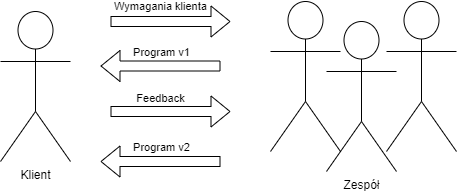
\includegraphics[scale=0.65]{przyklad1.png}
}

\frame{
	\frametitle{Charakterystyczne cechy XP}
	\centering
	
	\begin{itemize}
		\item Klient jest częścią zespołu, obie strony pozostają w ciągłym kontakcie.
		\item Brak dokumentacji projektu, skupienie na informacji zwrotnej od klienta.
		\item Małe, ale częste wydania wersji.
		\item Minimalizacja złożoności oprogramowania, rozwijanie go w miarę potrzeb.
		\item Programiści pracują w parach.
		\item XP stosowane jest głównie w małych i średniej wielkości projektach.
	\end{itemize}
}

%PODSTAWOWE WARTOŚCI XP
\section{Podstawowe wartości XP}
\frame{
	\frametitle{Podstawowe wartości programowania ekstremalnego}
	\centering
	\begin{itemize}
		\item Komunikacja
		\item Prostota
		\item Feedback
		\item Odwaga
	\end{itemize}
	
}

\frame{
	\frametitle{Komunikacja}
	\centering
	W programowaniu ekstremalnym nie wykorzystuje się zazwyczaj dokumentacji, 
	dlatego jednym z najważniejszych aspektów jest komunikacja nie tylko pomiędzy członkami zespołu,\\
	ale też z klientem.\\
	\vspace{1em}
	Celem XP jest przedstawienie założeń projektu w jak najprostszy sposób,
	dzięki czemu programiści mają spójną wizję.  
}

\frame{
	\frametitle{Prostota}
	\centering
	Budowanie systemów w prosty sposób.\\
	Unikanie złożoności, skupienie się na aktualnych potrzebach.\\
	Wykorzystywanie zasady KISS (\emph{'Keep It Simple, Stupid!'}).
}

\frame{
	\frametitle{Feedback}
	\centering
	Produkt rozwijany jest w krótkich iteracjach\\
	i dostarczany do klienta.\\
	Postępy pracy są oceniane przez klienta, a feedback wykorzystywany jest przy wprowadzaniu zmian.\\
	\vspace{1em}
	Ważnym aspektem jest zadawanie pytań, stąd istotna jest bliska kooperacja klienta i zespołu developerskiego.
}

\frame{
	\frametitle{Odwaga}
	\centering
	Umiejętność podejmowania decyzji.\\
	Szczerość w kontaktach między członkami zespołu i klientem.\\
}

%PRAKTYKI XP
\section{Praktyki XP}
\frame{
	\frametitle{Praktyki programowania ekstremalnego}
	\centering
	W sumie dwanaście praktyk w czterech obszarach.\\
	\vspace{1em}
	\textbf{Omawiane obszary:}
	\begin{itemize}
		\item Planowanie
		\item Projektowanie
		\item Programowanie
		\item Testowanie
	\end{itemize}
}

\frame{
	\frametitle{Planowanie}
	\centering
	W XP planowany jest wyłącznie krótki odcinek czasu w najbliższej przyszłości.\\
	\vspace{1em}
	Ze względu na to, że projekt długofalowo może wymagać zmian lub potrzeby klienta ulegną zmianie,\\
	proces planowania dotyczy tylko najbliższej iteracji.
}

\frame{
	\frametitle{Praktyki planowania}
	\centering
	\begin{itemize}
		\item Gra planistyczna - estymacja i określenie zakresu pracy na początku każdej iteracji.
		\item Metafora - przedstawienie projektu w jasny sposób, zrozumiały zarówno dla zespołu programistów, jak i klienta.
		\item Klient jako część zespołu - ciągły kontakt, udostępnianie klientowi najnowszej wersji tworzonego oprogramowania, feedback.
	\end{itemize}	
}

\frame{
	\frametitle{Projektowanie}
	\centering
	
	Projektowanie rozwiązań odbywa się tuż przed etapem projektowania ze względu na ich ścisłe powiązanie.\\
	Prostota projektu ma się przekładać na prostotę programowania. \\
	\vspace{1em}
	Brak dokumentacji wymaga jasnego i przejrzystego kodu, 
	który sam w sobie staje się dokumentacją. 
}

\frame{
	\frametitle{Praktyka projektowania}
	\centering
	
	\begin{itemize}
		\item Prostota - oprogramowanie projektowane w jak najprostszy możliwy sposób, usuwanie złożoności. 
	\end{itemize} 
}

\frame{
	\frametitle{Programowanie}
	\centering
	Najważniejszy etap w XP.\\
	\vspace{1em}
	Programowanie zajmuje najwięcej czasu\\
	i jest kluczowe dla projektu.
}

\frame{
	\frametitle{Praktyki programowania}
	\centering
	\begin{itemize}
		\item Częste wydania - nowe wersje dla klienta w krótkich odstępach czasowych.\\
		\item Refaktoryzacja - uporządkowanie struktury kodu, zachowanie spójności i klarowności.\\
		\item Standard kodowania - wspólne dla wszystkich programistów konwencje pisania kodu.\\
		\item Ciągła integracja - nowe funkcjonalności integrowane są jak najczęściej z całością systemu.\\
	\end{itemize}
}

\frame{
	\frametitle{Praktyki programowania}
	\centering
	\begin{itemize}
		\item Współwłasność kodu - każdy programista może dokonywać zmian w dowolnym miejscu i na dowolnym etapie rozwijania projektu.\\
		\item Brak nadgodzin - programiści pracują maksymalnie 40 godzin tygodniowo.\\
		\item Praca w parach - jedna osoba programuje, druga osoba sprawdza i sugeruje nowe rozwiązania.\\
	\end{itemize}
}

\frame{
	\frametitle{Testowanie}
	\centering
	Wykorzystywanie testów jednostkowych pisanych przez programistów w celu sprawdzenia poprawności ich kodu.\\
	\vspace{1em}
	Wykorzystywanie testów funkcjonalnych, sprawdzających poprawność funkcjonalności zleconych przez klienta.
}

\frame{
	\frametitle{Praktyka testowania}
	\centering
	\begin{itemize}
		\item Testowanie przed programowaniem - zautomatyzowane testy pisane są przed implementowaniem funkcjonalności. 
	\end{itemize}
}

%WADY I ZALETY
\section{Wady i zalety}
\frame{
	\frametitle{Zalety:}
	\centering
	\begin{itemize}
		\item Priorytetyzacja zadań, prostota, rozwijanie projektu "od ogółu do szczegółu".
		\item Krótkie iteracje i częstsze wydania, które przekładają się na szybszy feedback i wyłapywanie nieścisłości.
		\item Programowanie w zespołach dwuosobowych pozwala na szybsze rozwiązywanie problemów programistycznych.
		\item Poleganie na komunikacji werbalnej, co może być zaletą, ale...
	\end{itemize}
}

\frame{
	\frametitle{Wady:}
	\centering
	\begin{itemize}
		\item ...również wadą, ponieważ nie istnieje formalna dokumentacja.
		\item Dalsze rozwijanie projektu bez dokumentacji może okazać się problematyczne.
		\item Projektowanie rozwiązań biorąc pod uwagę tylko krótką perspektywę czasową, może skutować długiem technologicznym.
		\item Ciągła dostępność klienta w celu odpowiadania na pytania developerów bywa niemożliwa dla zleceniodawcy.
		\item Zespół programistów powinien wykazywać się umiejętnościami interpersonalnymi, pozwalającymi na ścisłą kooperację.
	\end{itemize}
}


%PODSUMOWANIE
\section{Podsumowanie}
\frame{
	\frametitle{Podsumowanie}
	\centering
	Programowanie ekstremalne pozwala na stworzenie w krótkim czasie kolejnych wersji produktu dla klienta.\\
	\vspace{1em}
	Wymaga jednak od zespołu dobrych umiejętności komunikacyjnych i technicznych, a od klienta zaangażowania w proces tworzenia.\\
}

\frame{
	\frametitle{Bibliografia:}

	K. Beck, \emph{Extreme Programming Explained: Embrace Change}, Addison-Wesley, 2018.\\
	\vspace{1em}
	D. Wells, \emph{Extreme Programming},  http://www.extremeprogramming.org (dostęp marzec 2022).\\
	\vspace{1em}
	A. Kolm, \emph{Zarządzanie projektami IT}, http://zarzadzanieprojektami.it/ (dostep marzec 2022).\\
}

\end{document}